% !TEX TS-program = xelatex
% !TEX encoding = UTF-8 Unicode
\documentclass{article}
\usepackage{civl}

% SEE: https://ctan.org/pkg/titlepages
\newcommand*{\titleGap}{\begingroup
\raggedleft
\vspace*{16\baselineskip}

\begin{tabularx}{\textwidth}{@{}rXr@{}}
    \textit{Fédération} & & \\
    \textit{Aéronautique} & & \multirow{2}{*}{} \\ \cline{2-3}
    \textit{Internationale} & & \\
\end{tabularx}

{\Huge CIVL GAP}\\
{\Huge Annex to Section 7A}\\
\vspace*{2\baselineskip}
{\Large Centralised Cross-Country Competition Scoring for}\\
{\Large Hang-Gliding and Paragliding}\\
{\Large Classes 1 to 5}\\
\vspace*{2\baselineskip}
2017 Edition\\
Effective 1st May, 2017\\
\vspace*{10\baselineskip}

\begin{tabularx}{\textwidth}{@{}rXr@{}}
    \textit{Maison du Sport International} & & \\
    \textit{Av. de Rhodanie 54} & & \\
    \textit{CH-1007 Lausanne} & & \\
    \textit{(Switzerland)} & & \\
    \textit{Tél. +41 (0)21 345 10 70} & & \\
    \textit{Fax +41 (0)21 345 10 77} & & \\
    \textit{E-mail: \href{mailto:sec@fai.org}{sec@fai.org}} & & \\
    \textit{Web: \href{www.fai.org}{www.fai.org}} & & \\
\end{tabularx}

\endgroup}

\import{}{footer}
\pagestyle{gen}

\begin{document}
\import{}{header}

% SEE: http://tex.stackexchange.com/questions/86249/maketitle-text-before-title
{\let\newpage\relax\titleGap}\thispagestyle{pageone}

\newpage
\vspace*{\fill}
\section*{FEDERATION AERONAUTIQUE INTERNATIONALE\\MSI – Avenue de Rhodanie 54 – CH-1007 Lausanne – Switzerland}
Copyright 2017\\\\
All rights reserved. Copyright in this document is owned by the Fédération
Aéronautique Internationale (FAI). Any person acting on behalf of the FAI or
one of its Members is hereby authorised to copy, print, and distribute this
document, subject to the following conditions:\\
\textbf{
    \begin{enumerate}
        \item
            The document may be used for information only and may not be
            exploited for commercial purposes.
        \item
            Any copy of this document or portion thereof must include this
            copyright notice.
        \item
            Regulations applicable to air law, air traffic and control in the
            respective countries are reserved in any event. They must be
            observed and, where applicable, take precedence over any sport
            regulations
    \end{enumerate}
}
Note that any product, process or technology described in the document may be
the subject of other Intellectual Property rights reserved by the Fédération
Aéronautique Internationale or other entities and is not licensed hereunder.

\newpage
\section*{RIGHTS TO FAI INTERNATIONAL SPORTING EVENTS}
All international sporting events organised wholly or partly under the rules of
the Fédération Aéronautique Internationale (FAI) Sporting Code
\footnote{FAI Statutes, ..........................................................................  Chapter 1, ...................para. 1.6}
are termed FAI International Sporting Events
\footnote{FAI Sporting Code, Gen. Section, ......................................... Chapter 4, ...................para 4.1.2}
. Under the FAI Statutes
\footnote{FAI Statutes, .......................................................................... Chapter 1, ...................para 1.8.1}
, FAI owns and controls all rights relating to FAI International Sporting
Events. FAI Members
\footnote{FAI Statutes, .......................................................................... Chapter 2, ...................para 2.1.1; 2.4.2; 2.5.2 and 2.7.2}
shall, within their national territories
\footnote{FAI By-Laws, ......................................................................... Chapter 1, ...................para 1.2.1}
, enforce FAI ownership of FAI International Sporting Events and require them
to be registered in the FAI Sporting Calendar
\footnote{FAI Statutes, .......................................................................... Chapter 2, ...................para 2.4.2.2.5}
.

An event organiser who wishes to exploit rights to any commercial activity at
such events shall seek prior agreement with FAI. The rights owned by FAI which
may, by agreement, be transferred to event organisers include, but are not
limited to advertising at or for FAI events, use of the event name or logo for
merchandising purposes and use of any sound, image, program and/or data,
whether recorded electronically or otherwise or transmitted in real time. This
includes specifically all rights to the use of any material, electronic or
other, including software, that forms part of any method or system for judging,
scoring, performance evaluation or information utilised in any FAI
International Sporting Event
\footnote{FAI By-Laws, ......................................................................... Chapter 1, ...................paras 1.2.2 to 1.2.5}
.

Each FAI Air Sport Commission
\footnote{FAI Statutes, .......................................................................... Chapter 5, ...................paras 5.1.1, 5.2, 5.2.3 and 5.2.3.3}
may negotiate agreements, with FAI Members or other entities authorised by the
appropriate FAI Member, for the transfer of all or parts of the rights to any
FAI International Sporting Event (except World Air Games events
\footnote{FAI Sporting Code, Gen. Section, ......................................... Chapter 4, ...................para 4.1.5}
) in the discipline
\footnote{FAI Sporting Code, Gen. Section, ......................................... Chapter 2, ...................para 2.2.}
, for which it is responsible
\footnote{FAI Statutes, .......................................................................... Chapter 5, ...................para 5.2.3.3.7}
or waive the rights. Any such agreement or waiver, after approval by the
appropriate Air Sport Commission President, shall be signed by FAI Officers
\footnote{FAI Statutes, .......................................................................... Chapter 6, ...................para 6.1.2.1.3}
.

Any person or legal entity that accepts responsibility for organising an FAI
Sporting Event, whether or not by written agreement, in doing so also accepts
the proprietary rights of FAI as stated above. Where no transfer of rights has
been agreed in writing, FAI shall retain all rights to the event. Regardless of
any agreement or transfer of rights, FAI shall have, free of charge for its own
archival and/or promotional use, full access to any sound and/or visual images
of any FAI Sporting Event. The FAI also reserves the right to arrange at its
own expense for any and all parts of any event to be recorded.

Editor’s note: Hang-gliding and paragliding are sports in which both men and
women participate. Throughout this document the words “he”, “him” or “his” are
intended to apply equally to either sex unless it is specifically stated
otherwise.

\newpage
Editor’s note: Hang-gliding and paragliding are sports in which both men and
women participate. Throughout this document the words “he”, “him” or “his” are
intended to apply equally to either sex unless it is specifically stated
otherwise.

\begin{tabularx}{\textwidth}{|l|l|X|}
 \hline
    \textbf{Revision} & \textbf{Author} & \textbf{Changes} \\
 \hline
 2014 R1.1 & Joerg Ewald & Correction of a number of typos \\
 \hline
 2015 R1.0 & Joerg Ewald & Added changes from the 2015 CIVL Plenary:
    \begin{itemize}
        \item Use same leading coefficient calculation for both hang gliding and paragliding
        \item Use QNH for altitude measurement
        \item Final glide decelerators in paragliding no longer mandatory
        \item Distance measurement based on WGS84 ellipsoid postponed
    \end{itemize} \\
 \hline
 2016 R1.0 & Joerg Ewald & Added changes from the 2016 CIVL Plenary:
    \begin{itemize}
        \item PG: Double the amount of available leading points (reducing time points accordingly)
        \item PG: If no pilot in goal, the leading points weight is proportional to the task distance covered by pilots, up to 100 points.
        \item HG: Jump the gun penalty is now one point for every 2 seconds (was for every 3 seconds).
    \end{itemize} \\
 \hline
 2016 R1.1 & Joerg Ewald & Correct Figures 6 and 7 (point allocation graphs) \\
 \hline
 2017 R1.0 & Elena Filonova & Made changes according to 2017 CIVL Plenary decisions related to Chapters 3,7,13,14. \\
\hline
\end{tabularx}

\newpage
\tableofcontents

\newpage
\section{Introduction}
This document contains all definitions required to score centralised
cross-country competitions for both hang-gliding and paragliding. Its main
purpose is to serve as an addendum to sections 7A and 7B of the FAI sporting
code. Additionally, it should serve as an educational tool for all parties
involved in such competitions, as a reference for the implementation of scoring
systems, as well as a basis for future improvements and modifications.

\subsection{Scope}
The document’s scope is restricted to scoring of FAI Category 1 cross-country
competitions for hang-gliding and paragliding: World and Continental
championships in both sports. CIVL’s rule setting targets these competitions
exclusively, whereas organisers of FAI Category 2 competitions as well as
non-sanctioned competitions are free to score their competitions however they
like. Most of them do follow CIVL’s lead, though, so this document should also
cover the majority of Category 2 events as well.

\subsection{Sources}
The remainder of this document is based on:
\begin{itemize}
\item “The GAP Guide” (2011 edition)
\item FAI Sporting Code Section 7A for Hang-Gliding (2013 edition)
\item FAI Sporting Code Section 7B for Paragliding (2013 edition)
\item The scoring implementation within CIVL’s scoring software, FS (aka “FScomp”)
\item Appendix C of the Paragliding World Cup Association’s 2013 Competition Rules
\end{itemize}

\subsection{Changes from previous edition}
Changes from the 2015 edition of this document will be marked with a vertical
sidebar.

\subsection{Differences between Hang-Gliding and Paragliding}
Initially, both hang-gliding and paragliding competitions used the same system
for scoring, generally known as “GAP”. But over time, through their two
separate sporting codes, the two disciplines introduced more and more changes
that would only apply to one, but not the other. This mainly in non-standard
situations such as stopped tasks, pilots landing just short of goal, or pilots
crossing the start line too early. Where not explicitly stated otherwise, the
contents of this document always apply to both disciplines. Definitions
applying only to one, but not the other, are clearly marked as such.

\begin{hg}
Text marked in blue applies exclusively to hang-gliding.
\end{hg}

\begin{pg}
Text marked in orange applies exclusively to paragliding.
\end{pg}

\newpage
\section{The GAP Philosophy}
CIVL’s scoring system is generally known as “GAP”, named after the first-name
initials of its three inventors Gerolf Heinrichs (G), Angelo Crapanzano (A) and
Paul Mollison (P). Their intention was to “create a fair scoring system easily
adaptable to any competition anywhere in the world, both for hang gliding and
paragliding, with a philosophy that is easy for the pilot to understand,
regardless of the mathematical complexity of the underlying formulas”.

\subsection{History}
Work on GAP started in 1998, and it was officially introduced in 2000, to allow
scoring of competitions based on GPS track logs, instead of photographic
evidence as it had been used until then.

In 2002, an updated version, named “GAP 2002” was published. This introduced
the concept of leading points, which are calculated by comparing the complete
track logs of all pilots in a task. Leading points replaced the departure
points used in GAP 2000

In 2005, a variation of GAP 2002 was introduced in Australia, named “OzGAP” or
“OzGAP 2005”. The difference to GAP lies mainly in the way arrival points are
calculated, but this was never adopted by CIVL.

In 2008, “GAP 2008” was officially released. The main scoring mechanisms
remained unchanged from the 2002 edition, but the implementation of GAP 2008
included several rules introduced in the sporting codes for either hang-gliding
or paragliding. These cover stopped tasks, starting too early, and landing
between the end of the speed section and goal.

In 2011, “GAP 2011” marked another software release where the main scoring
remained unchanged from the 2002 definition and implementation. The main
changes were all for paragliding: altitude bonus in stopped tasks, as well as
a reduced number of available points in stopped tasks and in tasks with no
pilots in goal.

In 2012, the “Jump the Gun” rule for early starts in hang-gliding competitions
changed in S7A. This was implemented in FS, but this was also released,
unfortunately, as “GAP 2011”.

The 2014 edition introduced a number of significant changes for paragliding,
a few of which also applied to hang gliding. The majority of those changes
originated from the Paragliding World Cup Association (PWCA), and 2014 was the
first time that both CIVL and PWCA scored their paragliding competitions using
the same formula. The changes were:
\begin{itemize}
    \item
        Nominal launch parameter, see~\ref{sec:nominal-launch} (hang gliding
        and paragliding)
    \item
        Final glide decelerator, see~\ref{sec:final-glide-decelerator}
        (paragliding)
    \item
        Goal shape, see~\ref{sec:goal-definition} (paragliding)
    \item
        Purely linear distance points, see~\ref{sec:distance-points}
        (paragliding)
    \item
        Adjusted formula for leading points, see~\ref{sec:leading-points}
        (paragliding)
    \item
        No more arrival points, see~\ref{sec:arrival-points} (paragliding)
    \item
        Scoring of stopped tasks, see~\ref{sec:stopped-tasks} (hang gliding and
        paragliding)
    \item
        Use of FTV for competition scoring,
        see~\ref{sec:overall-competition-ranking} (paragliding)
\end{itemize}
This 2015 edition applies the 2014 changes in leading points calculations for
paragliding now also to hang gliding. In paragliding, the use of final glide
deceleration methods is no longer mandatory. QNH is now used as the primary
altitude measurement. Distance calculations continue to be based on the FAI
sphere, the introduction of a new distance measurement regime, based on the
WGS84 ellipsoid, has been postponed.

2016: In Paragliding, the leading points weight (maximum available leading
points) is doubled compared to the previous version. This reduces the available
time points. Also, if no pilot is in goal, the weight is now calculated as the
ratio between task distance and actual distance covered by the pilot who flew
the furthest. The maximum in this case is 0.1 (equivalent to 100 points for
a task with task quality 1). In hang gliding, the penalty for jumping the gun
was increased for one point every three seconds to one point every 2 seconds.

\subsection{Scoring Process}
Scoring follows a nine-step process, as depicted in
Figure~\ref{fig:scoring-process}:

\begin{figure}[h!]
    \centering
    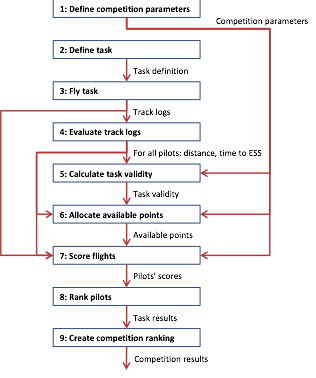
\includegraphics[scale=0.7]{img/scoring-process.png}
    \caption{Scoring process}
    \label{fig:scoring-process}
\end{figure}

\begin{enumerate}
    \item
        Setting the competition parameters, or “GAP parameters”, according to
        the competition site, the expected pilot level and the expected tasks.
        This happens once for each competition, at the outset, and must not be
        changed throughout the competition. See
        section~\ref{sec:use-of-tracklog-data}.
    \item
        Setting a task – this happens typically once per day on flyable days.
        See section~\ref{sec:task-setting}.
    \item
        Letting the pilots fly the task. See section~\ref{sec:flying-a-task}.
    \item
        Evaluating the task, by collecting all pilots’ track logs for this
        task, and determining for each pilot the distance flown and, if the end
        of speed section was reached, in what time this happened. See
        section~\ref{sec:task-evaluation}.
    \item
        Calculating the task validity based on the task’s statistical values
        such as fastest time to ESS, number of pilots in goal, average distance
        flown and several others. See section~\ref{sec:task-validity}.
    \item
        Points allocation: Calculating the maximum number of points awarded for
        distance, speed, leading and arrival, based on the task validity and
        the statistical values found in the task evaluation. See
        section~\ref{sec:points-allocation}.
    \item
        Scoring each pilot’s flight, by calculating the awarded points for
        distance, speed, leading and arrival. The outcome, the pilots’ total
        score, is the sum of these four values. See
        sections~\ref{sec:pilot-score} and ~\ref{sec:special-cases}.
    \item
        Ranking all pilots according to their total score for the task results.
        See section~\ref{sec:task-ranking}.
    \item
        Aggregation of task results for competition scoring and ranking. See
        section~\ref{sec:competition-ranking}.
\end{enumerate}

\newpage
\section{Definitions}
The definitions of flights, locations, distances and times of CIVL GAP are
described in Section 7A 5.2.1.
\begin{itemize}
    \item Flight
    \item Free flight
    \item Competition task
    \item Competition flight
    \item Take-off
    \item Speed section
    \item Start of speed section (SSS)
    \item Turnpoint (TP)
    \item Control zone
    \item End of speed section (ESS).
    \item Goal
    \item Landing place
    \item Task distance
    \item Flown distance
    \item Finish point
    \item Race start
    \item Start time
    \item Start gate
    \item Window open time
    \item Task deadline
    \item Finish time
    \item Task time
    \item Landing time
\end{itemize}


\newpage
\section{Use of Tracklog Data}
\label{sec:use-of-tracklog-data}
\subsection{Position}
Coordinates of positions, such as turn points or pilot positions, are always
given as WGS84 coordinates, based on the WGS84 ellipsoid. The coordinate format
is UTM by default, but other formats can be chosen by organisers as
appropriate.

\subsection{Distance}
\label{sec:distance}
In general, task evaluation occurs in the \(x/y\) plain, therefore distance
measurements are always exclusively horizontal measurements. The earth model used
is the FAI sphere, with a radius of 6371.0 km.

\begin{pg}
In paragliding, for final glide decelerators (\ref{sec:final-glide-decelerator})
and altitude bonus in stopped tasks (\ref{sec:distance-stopped-tasks}), altitude
is also considered, but this does not affect distance calculations between two
geographic points.
\end{pg}

\begin{hg}
In hang gliding, for altitude bonus in stopped tasks (\ref{sec:distance-stopped-tasks}),
altitude is also considered, but this does not affect distance calculations between
two geographic points.
\end{hg}

The distance between two points, identified by their radian coordinates
\(lat_1/long_1\) and \(lat_2/long_2\), is calculated using the Haversine formula.
\begin{align*}
    distLat &= lat_2 - lat_1 \\
    distLong &= long_2 - long_1 \\
    a &= \sin(\frac{distLat}{2})^2 + \cos lat_1 * \cos lat_2 * \sin(\frac{distLong}{2})^2 \\
    radianDistance &= 2 * \atantwo(\sqrt a, \sqrt{1 - a}) \\
    distance &= radianDistance * 6371000 \\
\end{align*}
To reproduce this formula in Excel, the following modification is necessary due
to a different implementation of the \(arctan2\) function:
\[ radianDistance = pi - 2 * \atantwo(\sqrt a, \sqrt{1 - a}) \]

\subsection{Altitude}
All altitude evaluation is primarily based on barometric altitude, as recorded
in the flight instrument tracklog (the International Standard Atmosphere
pressure altitude QNE) and then when necessary corrected by the scoring
software for the pressure conditions of the task (QNH). GNSS altitude may be
taken into consideration (from the primary tracklog or a backup log) only in
case of problems with barometric logging.

Category 2 Organisers may choose to use the less accurate GPS altitude instead
of barometric altitude.

\subsection{Time}
Time evaluation is based on GPS time, as given in GPS tracklogs. For better
readability, times of the day may be expressed in local time for the
competition location.

\newpage
\section{Competition Parameters}
Before the first task, the following parameters must be defined by the meet
director, or another person or group as defined by the competition’s local
regulations:
\begin{enumerate}
    \item Nominal Launch
    \item Nominal Distance
    \item Minimum Distance
    \item Nominal Goal
    \item Nominal Time
\end{enumerate}
The values set for these parameters define how each task’s validity is
calculated. They should therefore be chosen very carefully, considering the
realistic potential of the flying site. Setting the values too low will prevent
the formula from distinguishing between demanding, high quality tasks and
quick, easy low quality tasks which are sometimes the only option due to
weather conditions.

\begin{pg}
In paragliding competitions, the following must also be defined by the same
person or group who defines the first five competition parameters above:
\begin{enumerate}
    \setcounter{enumi}{5}
    \item Final glide decelerator
    \item Score-back time for stopped task
\end{enumerate}
\end{pg}

\subsection{Nominal Launch}
\label{sec:nominal-launch}
When pilots do not take off for safety reasons, to avoid difficult launch
conditions or bad conditions in the air, Launch Validity is reduced (see
section ~\ref{sec:launch-validity}). Nominal Launch defines a threshold as a percentage of the pilots
in a competition. Launch Validity is only reduced if fewer pilots than defined
by that threshold decide to launch.

The recommended default value for Nominal Launch is 96\%, which means that
Launch Validity will only be reduced if fewer than 96\% of the pilots present at
launch chose to launch.

\subsection{Nominal Distance}
Nominal distance should be set to the expected average task distance for the
competition. Depending on the other competition parameters and the distances
actually flown by pilots, tasks shorter than Nominal Distance will be devalued
in most cases. Tasks longer than nominal distance will usually not be devalued,
as long as the pilots fly most of the distance.

In order for GAP to be able to distinguish between good and not-so-good tasks,
and devalue the latter, it is important to set nominal distance high
enough\footnote{See also this excellent series of articles on the subject: Part
1: \url{http://ozreport.com/1360767307}; Part 2:
\url{http://ozreport.com/1360858575}; Part3:
\url{http://ozreport.com/1360944246}}.  

\subsection{Minimum Distance}
The minimum distance awarded to every pilot who takes off. It is the distance
below which it is pointless to measure a pilot's performance. The minimum
distance parameter is set so that pilots who are about to "bomb out" will not
be tempted to fly into the next field to get past a group of pilots – they all
receive the same amount of points anyway.

\subsection{Nominal Goal}
The percentage of pilots the meet director would wish to have in goal in
a well-chosen task. This is typically 20 to 40\%. This parameter has a very
marginal effect on distance validity (see section~\ref{sec:distance-validity}).

\subsection{Nominal Time}
Nominal time indicates the expected task duration, the amount of time required
to fly the speed section. If the fastest pilot’s time is below nominal time,
the task will be devalued. There is no devaluation if the fastest pilot’s time
is above nominal time.

Nominal time should be set to the expected “normal” task duration for the
competition site, and nominal distance / nominal time should be a bit higher
than typical average speeds for the area.

\begin{pg}
\subsection{Final Glide Decelerator}
\label{sec:final-glide-decelerator}
The concept of a final glide decelerator was introduced to counteract
a development in competition paraglider design which favoured stability at high
speeds over stability at trim speed. The two final glide decelerators available
are:
\begin{description}
    \item [Conical end of speed section (CESS)]
        Instead of a cylinder, the end of speed section is an inverted cone.
        Time stops for a pilot when they enter that cone. For details
        see~\ref{sec:define-CESS}.
    \item [Arrival altitude time bonus (AATB)]
        The time bonus is calculated based on each pilot’s altitude above goal
        when crossing the end of speed section cylinder. This bonus is then
        deducted from the pilot’s speed section time to determine the score
        time. See also~\ref{sec:time-for-speed-section}.
\end{description}
A meet director may choose to use no final glide decelerator, or use either of
the two outlined above.
\end{pg}

\begin{pg}
\subsection{Score-back Time}
\label{sec:score-back-time}
In a stopped task, this value defines the amount of time before the task stop
was announced that will not be considered for scoring. The default is
5 minutes, but depending on local meteorological circumstances, it may be set
to a longer period for a whole competition. See also section~\ref{sec:stop-task-time}.
\end{pg}

\newpage
\section{Task Setting}
\label{sec:task-setting}
\subsection{Definition of a task}
\label{sec:task-definition}
A task can be either a race task or an open distance task.

\subsubsection{Race task}
A race task definition consists of:
\begin{enumerate}
    \item A launch point, given as GPS coordinates
    \item A number of control zones
    \item A goal
    \item
        An indication which of the control zones is the start (start of speed
        section)
    \item
        If goal does not serve as end of speed section: An indication which of
        the control zones is the end of speed section, along with its specific
        parameters (such as incline and radius for CESS, altitude time bonus
        factor for AATB)
    \item A launch time window
    \item A start procedure, including timing
    \item Optionally, a task deadline
\end{enumerate}

\begin{pg}
In exceptional circumstances, with regard to restricted launch areas and poor
flying conditions, to ensure the task is fair for 2/3rds of the pilots, a task
may be run without leading/departure points. This is to be declared at the task
briefing.
\end{pg}

\subsubsection{Open distance task}
An open distance task definition consists of:
\begin{enumerate}
    \item A launch point, given as GPS coordinates
    \item A number of control zones
    \item Optionally, an indication which of the control zones is the start
    \item Optionally, a direction for the final, open distance leg
    \item A launch time window
    \item If a start control zone exists: A start time
    \item A task deadline
\end{enumerate}

\subsection{Definition of control zones}
Control zones are geographical areas which must be reached by the pilots in the
course of a task. The three types of control zones are the turnpoint cylinder,
the conical end of speed section and the goal semi-circle.

\subsubsection{Definition of a turnpoint cylinder}
A turnpoint cylinder is defined as:
\begin{enumerate}
    \item A centre point \(c\), given as GPS coordinates
    \item A radius \(r\), given in meters
    \item
        An indication whether the cylinder is an “exit” or an “enter” cylinder.
        This defines whether the corresponding turnpoint is considered reached
        by a pilot when crossing the cylinder’s boundary from its inside to the
        outside, or from its outside to the inside.
\end{enumerate}

A turnpoint cylinder is then given as the cylinder with radius \(r\) around the
axis which cuts the \(x/y\) plain orthogonally at the cylinder’s centre point
\(c\).  For task evaluation purposes, only the cylinder’s projection in the
\(x/y\) plain is considered: a circle of radius \(r\) around \(c\).

Note that for start cylinders (SSS), “enter” only makes sense if the following
turnpoint cylinder lies within the SSS cylinder. Likewise, an “exit” only makes
sense if the first turnpoint lies outside of the SSS cylinder. Currently, the
start direction cannot be set within FS. Instead the program automatically
scores according to this logic.

\subsubsection{Definition of conical end of speed section}
\label{sec:define-CESS}

\begin{figure}[h]
    \centering
    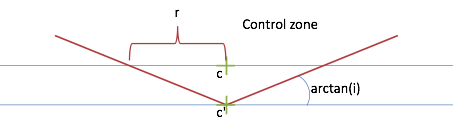
\includegraphics[scale=1]{img/conical-end.png}
    \caption{Conical end of speed section from the side}
\end{figure}

\begin{pg}
A conical end of speed section is defined as:
\begin{enumerate}
    \item A centre point \(c\), given as GPS coordinates and altitude
    \item
        An incline \(i\), given as a ratio of altitude/distance to the centre
        point
    \item
        A radius \(r\), indicating the size of the circle resulting from the
        intersection between the cone and a horizontal plane at goal altitude
\end{enumerate}

A conical end of speed section is given as the cone resulting from an axis of
inclination \(i\) through the centre point \(c'\), which is equal to point
\(c\), but has its altitude lowered by \(r/i\) metres compared to \(c\).  The
incline is chosen for each task. The default value is 1:3.5. Values suggested
for use are between
1:2.5 and 1:4.
\end{pg}
\subsection{Definition of goal}
\label{sec:goal-definition}
A goal can be
\begin{enumerate}
    \item A cylinder (enter or exit), see above, or
    \item A line, defined by:
    \begin{enumerate}
        \item A centre point \(c\), given as GPS coordinates
        \item A length \(l\), given in meters
    \end{enumerate}
\end{enumerate}

\begin{pg}
If CESS is used, goal must either be a line at the cone’s centre point,
a cylinder at the cone’s centre point with a radius smaller than radius r of
the cone definition, or be located at a point that is different from the cone’s
centre point.
\end{pg}

\subsubsection{Goal line}
\label{sec:goal-line}
\begin{figure}[h]
    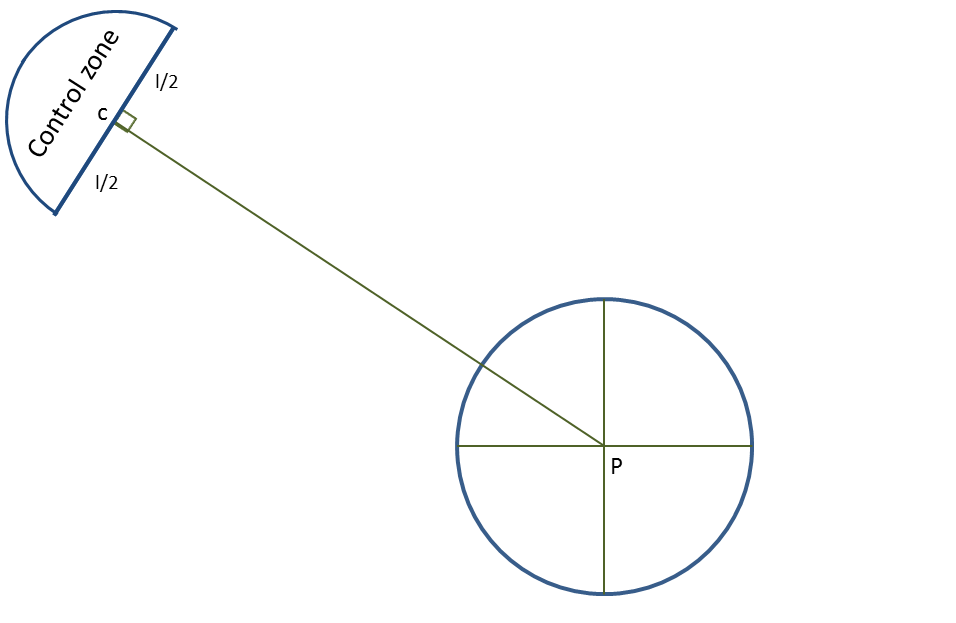
\includegraphics[scale=0.8]{img/goal-line.png}
    \caption{Goal line definition for paragliding}
\end{figure}

The goal control zone consists of the semi-circle with radius \(l/2\) behind
the goal line, when coming from the last turn point that is different from the
goal line centre. Entering that zone without prior crossing of the goal line is
equivalent to crossing the goal line.  Physical lines can be used in addition
to the official, virtual goal line as defined by GPS coordinates, to increase
attractiveness for spectators and media, and to increase visibility for pilots.
Physical lines must be at least 50m long and 1m wide, made of white material
and securely attached to the ground. The physical line must match as closely as
possible the corresponding virtual line as defined by the goal GPS coordinates
and the direction of the last task leg. It must not be laid out further from
the previous turn point than the goal GPS coordinates.

By default, the goal line length \(l\) is set to 400m.

\subsection{Start procedures}
Start procedures define how an individual pilot’s start time is determined.
A start can be either air- or ground-started, and it can be either a race to
goal or an elapsed time start.

\subsubsection{Air start}
For air-started tasks, the competitors are free to launch any time during the
launch window, and to fly about, regardless of any turnpoint or start
cylinders, up to their race start. Race start is defined as the crossing of the
start cylinder in the prescribed direction for the last time before continuing
to flying through the remainder of the task.

\subsubsection{Ground start}
In a ground-started task, the race starts with the pilots’ launch. Since
a launch can be difficult to detect from a GPS track, the task setters must set
a cylinder around the launch area as the first turnpoint. A pilot’s start is
registered when he exits this cylinder for the first time. In the case of
a race to goal task, the launch window open time is the same as the first (or
only) start gate time.

\subsubsection{Race to goal}
A race to goal start is defined by one or more so-called “start gates”. The
first – or only – start gate is given as a daytime. Subsequent start gates are
given as a time interval, along with the number of start gates.

\textit{Example 1: “We have a Race to Goal task, the start gate opens at 13:00”}

\textit{Example 2: “We have a Race to Goal task with 5 start gates from 13:30 at a 20
minutes interval.”} – the start gate times in this case are 13:30, 13:50, 14:10,
14:30, and 14.50.  Pilots are free to start any time after the first (or
single) start gate. A pilot’s start time is then defined as the time of the
last start gate after which he started flying the speed section of the task.

\textit{Example 3: Given the start gates from Example 2 above, pilot A, crossing the
start cylinder at 13:49:01, will be given a start time of 13:30. Any pilot
starting after 14:50 will be given a start time of 14:50.}

Starting before the first (or only) start gate is considered a failed start.
Some refer to this as “jumping the gun”. The two disciplines handle failed
starts differently, see section~\ref{sec:early-start}.

\subsubsection{Elapsed time}
An elapsed time start is defined by a single “start gate”, given as a daytime.
Pilots are free to start any time after this start gate. A pilot’s start time
is then defined as the time at which he started flying the speed section of the
task. Each pilot has therefore an individual start time.

\textit{Example 1: “We have an Elapsed Time task, the start gate opens at 12:30”}
– pilot A starting at 12:31:03 has a start time of 12:31:03, pilot B starting
at 15:48:28 has a start time of 15:48:28.

\subsection{Distances}
\subsubsection{Task distance}
\label{sec:task-distance}
Task distance is defined as the path of shortest distance from the start point
to goal that touches all turnpoint cylinders. The method to calculate this
distance is buried in FS’ code and will be documented at a later time.

Currently, this method mistreats the case where after ESS one or several
turnpoints have to be reached with centres different from ESS’ centre point:
The two legs to and from ESS are optimized for distance as well, which can
result in a longer last leg before ESS than what pilots experience in reality.
As a result, pilots can reach ESS with a shorter flown distance than what FS
indicates is the distance required to reach ESS. This only affects pilots
landing between ESS and goal, but does not represent a disadvantage to those
pilots. The speed section distance calculation used for scoring (see below) is
not affected by this.

\subsubsection{Speed section distance}
Speed section distance is defined as the path of shortest distance from start
of speed section to end of speed section that touches all turnpoint cylinders.
The method to calculate this distance is the same as for task distance.

\newpage
\section{Flying a task}
\label{sec:flying-a-task}
There are 2 task types: race task and open distance task. The definitions are
given in Section 7A-5.2.2.

\newpage
\section{Task evaluation}
\label{sec:task-evaluation}
From each pilot’s track, task evaluation determines the distance this pilot
flew along the task, and the time this pilot took to fly the speed section.

\subsection{Reaching a control zone}
\subsubsection{Reaching a turnpoint cylinder}
\label{sec:reaching-a-turnpoint-cylinder}
A cylinder is considered “reached” by a pilot if that pilot’s track log shows
the pilot crossing out of the cylinder in the case of an exit cylinder, or into
the cylinder in case of an enter cylinder, by containing at least one track
point closer to the cylinder’s centre than the cylinder radius (enter) or
further away from the cylinder’s centre than the cylinder radius (exit). During
task evaluation, only the \(x/y\) coordinates are considered, and a point must
lie within (enter) or outside of (exit) the circle representing the turnpoint
cylinder in the \(x/y\) plain. This is determined by measuring the distance
between a track point and the turnpoint. This distance must be greater (exit)
or smaller (enter) than the cylinder’s radius.  To compensate for different
distance calculations and different earth models in use by today’s GPS devices
(FAI sphere vs. WGS84 ellipsoid), a 0.5\% tolerance is used for this
calculation. This had to be introduced so that a pilot reading the distance to
the next cylinder centre from his GPS device can rely on having reached the
turnpoint when the distance displayed by the instrument is smaller than the
defined turnpoint cylinder radius.

For enter cylinders, this means that a tracklog point that is closer to the
turnpoint than \(r*1.005\) is considered proof of reaching the turnpoint. For
exit cylinders, this means that a tracklog point that is further away from the
turnpoint than \(r*0.995\) is considered proof of reaching the turnpoint.
Starting January 1st, 2015 – provided all distance measurements are then based
on the WGS84 ellipsoid (see~\ref{sec:distance}) – the tolerance for turnpoint
cylinders in CIVL’s FAI Category 1 events will be reduced to 0.01\% of the
cylinder radius, with a minimum of 5 meter. Organisers of FAI Category 2 events
may continue using the existing 0.5\% tolerance, to accommodate pilots flying
with instruments which calculate distance based on the FAI sphere.

The time when a control zone was reached is determined by the time a so-called
“crossing” occurred. A crossing is defined as a pair of consecutive track
points, of which at least one lies inside the band determined by the
turnpoint’s centre, its radius and the tolerance value.
\begin{align*}
    tolerance &= 0.5\% | 0.01\% \\
    minTolerance &= 0m | 5m \\
    turpoint_i : innerRadius_i &= \min(radius_i * (1 - tolerance), radius_i - minTolerance) \\
    turpoint_i : outerRadius_i &= \max(radius_i * (1 + tolerance), radius_i + minTolerance) \\
\end{align*}
\begin{equation*}
    crossing_i = \exists_j (a \land b) \lor (c \land d)
\end{equation*}
\begin{align*}
    a = distance(center_i, trackpoint_j) &>= innerRadius_i \\
    b = distance(center_i, trackpoint_{j+1}) &<= outerRadius_i \\
    c = distance(center_i, trackpoint_j) &<= outerRadius_i \\
    d = distance(center_i, trackpoint_{j+1}) &>= innerRadius_i \\
\end{align*}
The time of a crossing depends on whether it actually cuts across the actual
cylinder, or whether both points lie within the tolerance band, but on the same
side of the actual cylinder.
\begin{align*}
    crossing . time &= trackpoint_{j+1} . time \ when \ A \\
    crossing . time &= trackpoint_j . time \ when \ B \\
    crossing . time &= interpolateTime(trackpoint_{j+1}, trackpoint_{j+1}) . time \ when \ C \\
\end{align*}
\begin{align*}
    A &= (a \land b) \lor (c \land d) \land turnpoint_i = ESS \\
    B &= (a \land b) \lor (c \land d) \land turnpoint_i \neq ESS \\
    C &= (a \land d) \lor (c \land b) \\
    \\
    a = distance(center_i, trackpoint_j) &< radius_i \\
    b = distance(center_i, trackpoint_{j+1}) &< radius_i \\
    c = distance(center_i, trackpoint_j) &> radius_i \\
    d = distance(center_i, trackpoint_{j+1}) &> radius_i \\
\end{align*}
The method used to interpolate the crossing time is buried in FS’ code and will
have to be documented at a later point.

Finally, given all n crossings for a turnpoint cylinder, sorted in ascending
order by their crossing time, the time when the cylinder was reached is
determined.
\begin{align*}
    turnpoint_i &= SSS : reachingTime_i = crossing_n . time \\
    turnpoint_i &\neq SSS : reachingTime_i = crossing_0 . time
\end{align*}
\subsection{Reaching a conical end of speed section}
\begin{pg}
A conical end of speed section is considered “reached” by a pilot if that
pilot’s track log contains at least one point where the required glide angle to
the cone’s centre point is equal to or smaller than the cone’s incline.
\begin{align*}
    crossing_i : \exists j : \\
    \frac{trackpoint_j . altitude - center_{CESS} . altitude}{center_{CESS}, trackpoint_{j}} \leq incline \\
    \land \frac{trackpoint_{j - 1} . altitude - center_{CESS} . altitude}{distance(center_{CESS}, trackpoint_{j - 1})} > incline \\
    \\
    crossing_i . time &= interpolateTime(trackpoint_{j + 1}, trackpoint_{j + 1})
\end{align*}
Given all n crossings for a CESS, sorted in ascending order by their crossing
time, the time when CESS was reached is determined.
\[ reachingTime_{CESS} = crossing_0 . time \]
If goal is at the CESS centre point, and a pilot reaches goal without
previously entering the CESS, he is considered having reached CESS at the time
when he crossed the goal line.
\end{pg}

\subsection{Reaching goal}
\subsubsection{Goal cylinder}
Verification of a pilot reaching a goal cylinder is achieved by the same method
as verification of reaching a turnpoint cylinder (~\ref{sec:reaching-a-turnpoint-cylinder})

\subsubsection{Goal line}
To reach goal in the case of a goal line, the goal line must be crossed in
flight. This is achieved when a line drawn between two adjacent points in the
pilot’s tracklog crosses the goal line in the correct direction.

\begin{pg}
Entering the goal control zone (semi-circle behind the goal line,
see~\ref{sec:goal-line}) from any direction without prior crossing of the goal
line is equivalent to crossing the goal line.
\end{pg}

If a physical line is used, crossing either the virtual or the physical goal
line counts as having reached goal. An official observation (through a goal
marshal or similar) of a pilot crossing the line in flight overrules a negative
goal crossing decision based on the pilot’s tracklog. Not crossing a physical
goal line for obvious safety reasons must be considered in the pilots’ favour.

\begin{hg}
The physical goal line is crossed when the hang glider’s nose cuts the line, in
the correct direction, before a landing is made.
\end{hg}

\begin{pg}
The physical goal line is crossed when the paraglider pilot’s leading foot cuts
the line, in the correct direction, before a landing is made.
\end{pg}

\subsection{Flown distance}

\subsubsection{Race task}
\label{sec:race-task}
To determine a pilot’s flown distance, a first step determines which turnpoints
he reached considering all timing restrictions: launch within launch time
window, valid start, but only until the task deadline time. After the last
turnpoint the pilot reached, for every remaining track point, the shortest
distance to goal is calculated using the method described in section
\ref{sec:task-distance}. The flown distance is then calculated as task distance
minus the shortest distance the pilot still had to fly. Therefore, for scoring,
the pilot’s best distance along the course line is considered, regardless of
where the pilot landed in the end.

If a pilot flies less than minimum distance, he will be scored for this minimum
distance. This also applies to pilots who are not able to produce a valid GPS
tracklog, but for whom launch officials verify launch within the launch window.

If a pilot reaches goal, he will be scored for the task distance.
\begin{align*}
    \forall p : p \in PilotsLandingBeforeGoal : bestDistance_p &= \max(minimumDistance, taskDistance - shortest) \\
    shortest &= \min(\forall track_p . point_i shortestDistanceToGoal(track_p . point_i))) \\
    \forall p : p \in PilotsReachingGoal : bestDistance_p &= taskDistance
\end{align*}

\subsubsection{Open distance task}
In an open distance task, if a pilot lands before the last of any given control
zones, his flown distance is calculated according to \ref{sec:race-task}. For
pilots flying further than the last control zone, the flown distance is
calculated by adding the pilot’s best distance flown in the open distance part
of the task (after the last control zone) to task distance between launch and
the last control zone. If the task gave a direction for the open distance leg,
then the pilot’s best distance projected onto that direction is considered.

\subsection{Time for speed section}
\label{sec:time-for-speed-section}
The time a pilot took to fly the speed section is determined by his start time
(which is influenced by the task’s start procedure and the time he crossed the
start of speed section cylinder) and the time when he crossed the end of speed
section after reaching all previous turn points. The smallest unit for time
measurement is one second.

Pilots who do not reach the end of speed section cylinder do not get a time.
\begin{align*}
    \forall p : p \in PilotsReachingESS : time_p &= timeAtESS_p - startTime_p
\end{align*}

\begin{pg}
If AATB is used, pilots receive a time bonus for their altitude above goal when crossing the ESS cylinder.
The number of seconds they receive for each meter is expressed by the ATTB factor.

By default, the ATTB factor is \(0.45 \ s/m\). Values suggested for use are between \(0.2 \ s/m\) and \(0.7 \ s/m\).
\begin{align*}
    \forall p : p \in PilotsReachingESS \\
    arrivalAltitudeTimeBonus_p &= (crossing_{p.ESS} . altitude - goal . altitude) * ATTBfactor \\
    time_p &= timeAtESS_p - startTime_p - arrivalAltitudeTimeBonus_p
\end{align*}
\end{pg}

\newpage
\section{Task Validity}
\label{sec:task-validity}
The task validity is a value between 0 and 1 and measures how suitable
a competition task is to evaluate pilots’ skills. It is calculated for each
task after the task has been flown, by multiplying the three validity
coefficients: Launch validity, distance validity, and time validity.
\begin{equation*}
    TaskValidity = LaunchValidity * DistanceValidity * TimeValidity
\end{equation*}

\subsection{Launch Validity}
\label{sec:launch-validity}
Launch validity depends on nominal launch and the percentage of pilots actually
present at take-off who launched. If the percentage of pilots on take-off who
launch is equal to nominal launch, or higher, then launch validity is 1. If,
for example, only 20\% of the pilots present at take-off launch, launch
validity goes down to about 0.1.

The reasoning behind launch validity: Launch conditions may be dangerous, or
otherwise unfavourable.  If a significant number of pilots at launch think that
the day is not worth the risk of launching, then the gung-ho pilots who did go
will not get so many points. This is a safety mechanism.

‘Pilots present’ are pilots arriving on take-off, with their gear, with the
intention of flying. For scoring purposes, ‘Pilots present’ are all pilots not
in the ‘Absent’ status (ABS): Pilots who took off, plus pilots present who did
not fly (DNF). DNFs need to be attributed carefully. A pilot who does not
launch due to illness, for instance, is not a DNF, but an ABS.
\begin{align*}
    LVR &= \min(1, \frac{NumberOfPilotsFlying}{NumberOfPilotsPresent * NominalLaunch}) \\
    LaunchValidity &= 0.027 * LVR + 2.917 * LVR^2 - 1.944 * LVR^3
\end{align*}

\begin{figure}[h!]
    \centering
    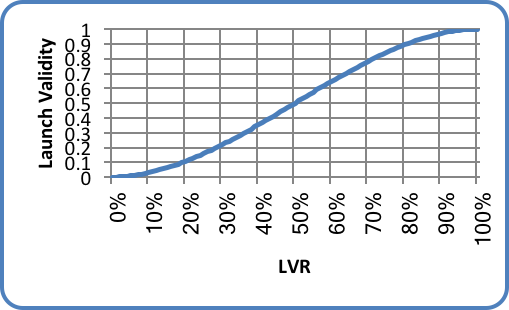
\includegraphics{img/launch-validity.png}
    \caption{Launch validity curve}
\end{figure}

\subsection{Distance Validity}
\label{sec:distance-validity}
Distance validity depends on nominal distance, nominal goal, the longest
distance flown and the sum of all distances flown beyond minimum distance. If
the task distance is quite short in relation to nominal distance, the day is
probably not a good measure of pilot skill because there would not be many
decisions to make.

If a task is longer than nominal distance, the day will not be devalued because
of distance validity, even if the nominal goal parameter value is not achieved,
as long as a fair percentage of pilots fly a good distance. This sounds like
a vague statement, but the task setter should try to set tasks that are
reasonable for the day and achievable. If everyone lands in goal, you must ask
if this was a valid test of skill - it probably was if the fastest time and the
distance flown were reasonably long. If everyone lands short of goal, was it an
unsuitable task but still a good test of pilot skill? You also can have the
case where a task that is shorter than nominal distance, has a distance
validity of almost 1. This will happen when a large percentage of the pilots
fly a large percentage of the course but, in this case, you still have
a practical devaluation because there will be little spreading between pilots’
scores.

In the formula below, \(p\) denotes an individual pilot.
\begin{align*}
    SumOfFlownDistancesOverMinDist &= \sum_p \max(0, FlownDist_p - MinDist) \\
    NominalDistanceArea &= \frac{(a + b)}{2} \\
    a &= (NomGoal + 1) * (NomDist - MinDist) \\
    b &= \max(0, NomGoal * (BestDist - NomDist) \\
    DVR &= \frac{SumOfFlownDistancesOverMinDist}{NumberOfPilotsFlying * NominalDistanceArea} \\
    DistanceValidity &= \min(1, DVR)
\end{align*}

\subsection{Time Validity}
Time validity depends on the fastest time to complete the speed section, in
relation to nominal time. If the fastest time to complete the speed section is
longer than nominal time, then time validity is always equal to 1.

If the fastest time is quite short, the day is probably not a good measure of
pilot skill because there would not be many decisions to make and, because of
this, luck can distort scores as there will be little possibility to recover
any accidental loss of time.

If no pilot finishes the speed section, then time validity is not based on time
but on distance: The distance of the pilot who flies the furthest in relation
to nominal distance is then used to calculate the time validity the same way as
if it was the time.
\begin{align*}
    if \ one \ pilot \ reached \ ESS \\
    TVR &= \min(1, \frac{BestTime}{NominalTime}) \\
    if \ no \ pilot \ reached \ ESS \\
    TVR &= \min(1, \frac{BestDistance}{NominalDistance}) \\
    TimeValidity &= \max(0, \min(1, -0.271 + 2.912 * TVR - 2.098 * TVR^2 + 0.457 * TVR^3))
\end{align*}

\begin{figure}[h!]
    \centering
    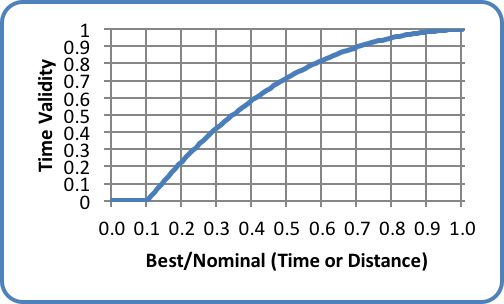
\includegraphics{img/time-validity.png}
    \caption{Time validity curve}
\end{figure}

\newpage
\section{Points Allocation}
\label{sec:points-allocation}
The available points for each task are \(1000*TaskValidity\). These points are
distributed between distance points, time points, leading points and arrival
points. The distribution depends on the percentage of pilots who reached goal
before the task deadline, compared to pilots who launched, as well as the
chosen goal form. It is expressed in terms of weight factors for each of the
four point categories: Distance weight, time weight, leading weight and arrival
weight. Weight factors are always between 0 and 1. A weight factor of 0.5 for
distance, for example, means that 50\% of the day’s available overall points
are available for distance points.
\begin{align*}
    GoalRatio &= \frac{NumberOfPilotsInGoal}{NumberOfPilotsFlying} \\
    DistanceWeight &= 0.9 - 1.665 * GoalRatio + 1.713 * GoalRatio^2 - 0.587 * GoalRatio^3 \\
    \hgh{LeadingWeight} &= \frac{1 - DistanceWeight}{8} * 1.4 \\
    \pgh{GoalRatio = 0 : LeadingWeight} &= \frac{BestDistance}{TaskDistance} * 0.1 \\
    \pgh{GoalRatio > 0 : LeadingWeight} &= \frac{1 - DistanceWeight}{8} * 1.4 * 2 \\
    \hgh{ArrivalWeight} &= \frac{1 - DistanceWeight}{8} \\
    \pgh{ArrivalWeight} &= 0 \\
    TimeWeight &= 1 - DistanceWeight - LeadingWeight - ArrivalWeight \\
    AvailableDistancePoints &= 1000 * TaskValidity  DistanceWeight \\
    AvailableTimePoints &= 1000 * TaskValidity * TimeWeight \\
    AvailableLeadingPoints &= 1000 * TaskValidity * LeadingWeight \\
    AvailableArrivalPoints &= 1000 * TaskValidity * ArrivalWeight
\end{align*}

\begin{figure}[h]
    \centering
    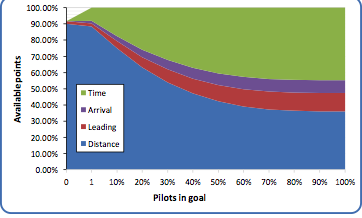
\includegraphics[scale=0.8]{img/points-allocation-hg.png}
    \caption{Points allocation for hang gliding}
\end{figure}

\begin{figure}[h]
    \centering
    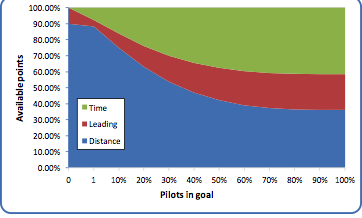
\includegraphics[scale=0.8]{img/points-allocation-pg.png}
    \caption{Points allocation for paragliding}
\end{figure}

\begin{hg}
From the above it follows that in hang-gliding, if nobody reaches ESS, then
a maximum of 900 points are available for distance and 18 points for leading
but, of course, no points for time nor arrival. This is also the maximum
possible number of points for an open distance task.
\end{hg}

\begin{align*}
    numberOfPilotsAtESS = 0 : \\
    \\
    AvaliableDistancePoints &= 1000 * TaskValidity * DistanceWeight \\
    AvailableTimePoints &= 0 \\
    AvailableLeadingPoints &= 1000 * TaskValidity * LeadingWeight \\
    AvailableArrivalPoints &= 0 \\
    \max(AvailableDistancePoints) &= 900 \\ 
    \max(availableLeadingPoints) &= 18 \\
    \max(availableTotalPoints) &= 918
\end{align*}

\newpage
\section{Pilot score}
\label{sec:pilot-score}
Each pilot’s score is the sum of that pilot’s distance, time, leading and
arrival points, rounded to the nearest whole number, 0.5 being rounded up.
\[ \forall p : p \in PilotsLaunched : TotalScore_p = DistancePoints_p + TimePoints_p + LeadingPoints_p + ArrivalPoints_p \]
\subsection{Distance points}
\label{sec:distance-points}
The distance considered for each pilot to calculate distance points is that
pilot’s best distance along the course line, up until the pilot landed or the
task deadline was reached, whichever comes first.

\begin{hg}
One half of the available distance points are assigned to each pilot linearly,
based on the pilot’s distance flown in relation to the best distance flown in
the task. The other half is assigned taking into consideration the difficulty
of the kilometers flown.
\begin{align*}
    LinearFraction_p &= \frac{Distance_p}{2 * BestDistance} \\
    i_p &= \lfloor Distance_p * 10 \rfloor \\
    DifficultyFraction_p &= DiffScore_{i_p} + ((DiffScore_{i_{p + 1}} - DiffScore_{i_p}) * (Distance_p * 10 - i_p)) \\
    DistancePoints_p &= (LinearFraction_p + DifficultyFraction_p) * AvailableDistancePoints
\end{align*}
\end{hg}

\begin{pg}
In the case of a stopped task, a pilot’s distance may be increased by an
altitude bonus (see~\ref{sec:distance-stopped-tasks}). The available distance
points are assigned to each pilot linearly, based on the pilot’s distance flown
in relation to the best distance flown in the task.
\[ DistancePoints_p = \frac{Distance_p}{BestDistance} * AvailableDistancePoints \]
\end{pg}

\subsubsection{Difficulty calculation}
\label{sec:difficulty-calculation}
\begin{hg}
To measure the relative difficulty of each 100 meters of the task, we consider
the number of pilots who landed in the successive few kilometers, and the
distance flown.

In a first step, for each 100-meter section of the task, the number of pilots
who landed in that section is counted. Pilots who landed before minimum
distance are counted as having landed at minimum distance. Only pilots who
landed out are considered for this calculation, pilots who reached goal are not
counted.
\begin{align*}
    \forall i : i < \lfloor MinDist * 10 \rfloor : PilotsLanded_i &= 0 \\
    PilotsLanded_{\lfloor MinDist * 10 \rfloor} &= \sum_{\forall Pilot : \lfloor PilotDistance * 10 \rfloor \leq \lfloor MinDist * 10 \rfloor} 1 \\
    \forall i : i > \lfloor MinDist * 10 \rfloor \land i \leq \lfloor MaxDist * 10 \rfloor : PilotsLanded_i &= \sum_{\forall q : q \in PilotsLandedOut : \lfloor Distance_q * 10 \rfloor = i} 1
\end{align*}
Then the difficulty for each 100-meter section of the task is calculated by
counting the number of pilots who landed further along the task. If 100 pilots
land out on a flight of 100 km, the next 3 km are considered. If 10 pilots land
out in 100 km, the next 30 km are considered. The variable LookAheadDist
contains the number of 100 meter slots to look ahead for this.
\begin{align*}
    LookAheadDist &= \max(30, round(\frac{30 * BestDistanceFlown}{NumberOfPilotsLandedOut}, 0)) \\
    \forall i : i < \lfloor MinDist * 10 \rfloor : Difficulty_i &= \sum_{j = i}^{j = \min(i + LookAheadDist, \lfloor BestDistanceFlown * 10 \rfloor)} PilotsLanded_j \\
    SumOfDifficulty = \sum_i Difficulty_i
\end{align*}
Relative difficulty is then calculated by dividing each 100-meter slot’s difficulty by twice the sum of all
difficulty values.
\[ \forall i : i \leq \lfloor MaxDist * 10 \rfloor : RelativeDifficulty_i = \frac{Difficulty_i}{2 * SumOfDifficulty} \]
Finally, we can calculate the difficulty score percentage for each 100-meter slot.
\begin{align*}
    \forall i : i < \lfloor MinDist * 10 \rfloor : DiffScore_i &= \sum_{j = 0}^{j = \lfloor MinDist * 10 \rfloor)} RelativeDifficulty_j \\
    \forall i : i > \lfloor MinDist * 10 \rfloor \land i < \lfloor BestDistanceFlown * 10 \rfloor : DiffScore_i &= \sum_{j = 0}^{j = i} RelativeDifficulty_j \\
    \forall i : i \geq \lfloor BestDistanceFlown * 10 \rfloor : DiffScore_i &= 0.5
\end{align*}
\end{hg}

\begin{pg}
The difficulty calculation does not apply to paragliding.
\end{pg}

\subsubsection{Example for difficulty calculation}
For an example of how the difficulty calculation works, see Figure 8: Note how
the slope of the green curve (the total Distance points) becomes steeper before
an area where many pilots landed and flatter just after. The red circles show
these areas before the big group at the 41 km mark, and after the 46 km mark.
There are two reasons for this:
\begin{enumerate}
    \item For safety and retrieval reasons, we do not want to encourage pilots to fly only a short distance past a group of landed pilots.
    \item If a pilot lands somewhere, he or she probably got into trouble just before, and then glided a while before landing.
\end{enumerate}

\begin{figure}[h]
    \centering
    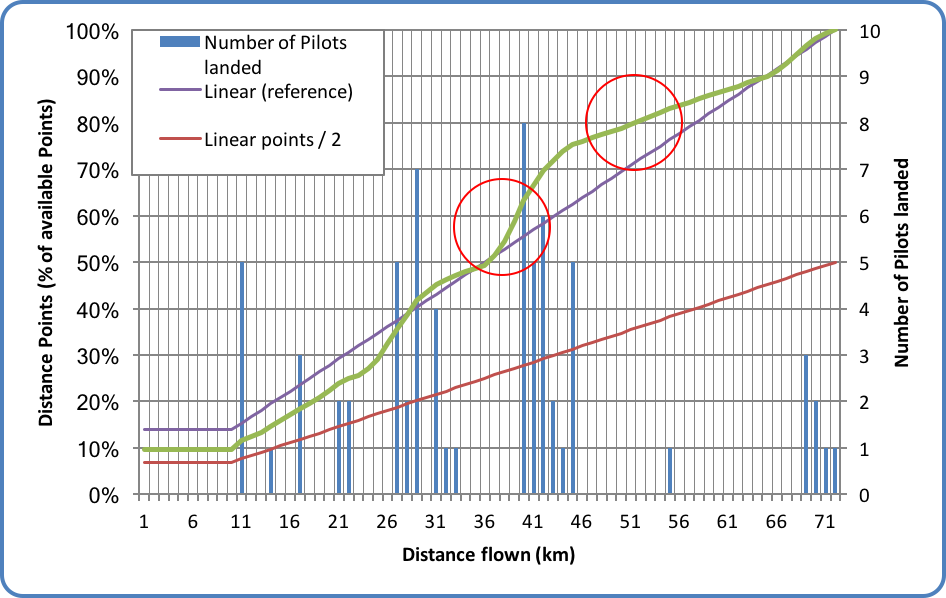
\includegraphics[scale=0.8]{img/distance-points.png}
    \caption{Sample Distance Points}
\end{figure}

\subsection{Time points}
Time points are assigned to the pilot as a function of best time and pilot time
– the time the pilot took to complete the speed section. Slow pilots will get
zero points for speed if their time to complete the speed section is equal to
or longer than the fastest time plus the square root of the fastest time. All
times are measured in hours.
\begin{align*}
    SpeedFraction_p &= \max(0, 1 - \sqrt[3]{\frac{Time_p - BestTime}{\sqrt{BestTime}}}^2) \\
    TimePoints_p &= SpeedFraction_p * AvailableTimePoints
\end{align*}

\textit{Examples}

For three examples of Time Point distributions for tasks with different best
times, see Figure~\ref{fig:time-points} and Table~\ref{tab:time-points}.

\begin{table}[h!]
    \begin{tabularx}{\textwidth}{|r|r|r|R|}
    \hline
        \textbf{Fastest Time} & \textbf{80\% Time Points time} & \textbf{50\% Time Points time} & \textbf{0 Time Points time} \\
    \hline
        1:00 & 1:05 & 1:21 & 2:00 \\
    \hline
        2:00 & 2:08 & 2:30 & 3:24 (3.4 hours) \\
    \hline
        3:00 & 3:09 & 3:37 & 4:42 (4.7 hours) \\
    \hline
    \end{tabularx}
    \caption{Sample time points distribution (all times in hours:minutes)}
    \label{tab:time-points}
\end{table}

\begin{figure}[h]
    \centering
    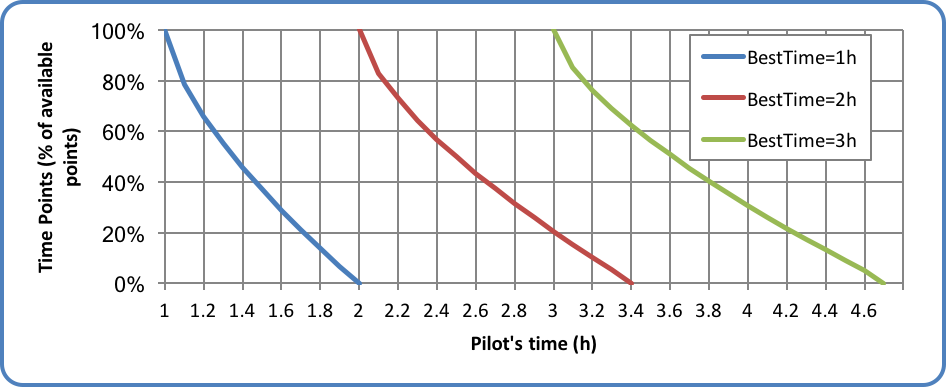
\includegraphics[scale=0.8]{img/time-points.png}
    \caption{Sample time point distributions}
    \label{fig:time-points}
\end{figure}


\subsection{Leading points}
\label{sec:leading-points}
Leading points are awarded to encourage pilots to start early and to reward the
risk involved in flying in the leading group. Pilots will get leading points
even if they landed before goal or the end of speed
section.
\begin{align*}
    LC_{min} &= \min(\forall p : p \in PilotsFlown : LC_p) \\
    LeadingFactor_p &= \max(0, 1 - \sqrt[3]{\frac{LC_p - LC_{min}}{\sqrt{LC_{min}}}}^2) \\
    LeadingPoints_p &= LeadingFactor_p * AvailableLeadingPoints
\end{align*}
To get an impression of the way leading points are awarded depending on a task’s minimal leading
coefficient, see Figure~\ref{fig:leading-points}.

\begin{figure}[h]
    \centering
    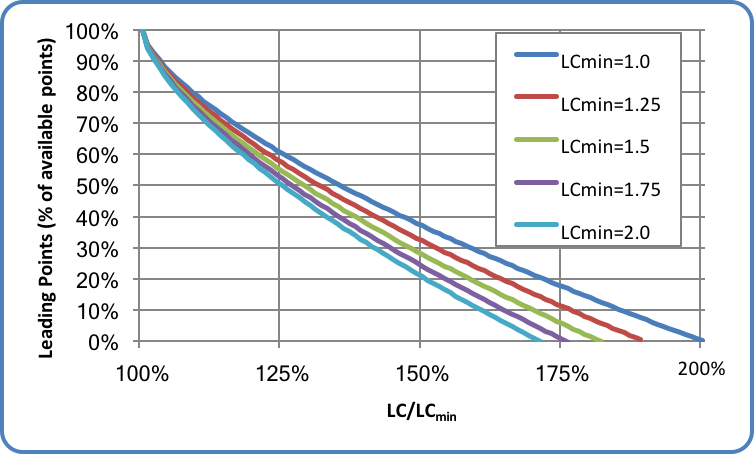
\includegraphics[scale=0.8]{img/leading-points.png}
    \caption{Leading points for various \(LC_{min}\)}
    \label{fig:leading-points}
\end{figure}

\subsubsection{Leading coefficient}
Each started pilot’s track log is used to calculate the leading coefficient
(LC), by calculating the area underneath a graph defined by each track point’s
time, and the distance to ESS at that time. The times used for this calculation
are given in seconds from the moment when the first pilot crossed SSS, to the
time when the last pilot reached ESS. For pilots who land out after the last
pilot reached ESS, the calculation keeps going until they land. The distances
used for the LC calculation are given in kilometers and are the distance from
each point’s position to ESS, starting from SSS, but never more than any
previously reached distance. This means that the graph never “goes back”: even
if the pilot flies away from goal for a while, the corresponding points in the
graph will use the previously reached best distance towards ESS.

Calculation of the leading coefficient (LC) for each pilot follows this
formula:
\begin{align*}
    LC_p &= \\
    \frac{\sum_{i : tp_i \in TrackPointsInSS_p} taskTime(tp_i) * (bestDistToESS(tp_{i - 1})^2 - bestDistToESS(tp_i)^2)}{1800 * LengthOfSpeedSection^2} \\
    \\
    \forall p : p \in PilotsLandedOut \land taskTime(tp_{max}) < ESSTime_{LastPilotAtESS} : LC_p &= \\
    LC_p + LastTime_{LastPilotAtESS} * bestDistToESS(tp_{max})^2 \\
    \\
    \forall p : p \in PilotsLandedOut \land taskTime(tp_{max}) \geq ESSTime_{LastPilotAtESS} : LC_p &= \\
    LC_p + taskTime(tp_{max}) * bestDistToESS(tp_{max})^2 \\
    \\
    taskTime(tp) &= \\
    \min(TaskDeadline, time(tp)) \\
    \\
    bestDistToESS(tp_0) &= \\
    LengthOfSpeedSection \\
    \\
    \forall i : i > 0 \land tp_i \in TrackPointsInSS_p : bestDistToESS(tp_i) &= \\
    \min(bestDistToESS(tp_{i - 1}), LenghtOfSpeedSection - distanceFlown(tp_i))
\end{align*}
\begin{pg}
In tasks where CESS is used, the CESS’s centre point is considered the last
point of the speed section. For LC calculations, any pilot crossing into the
CESS’s cone is immediately awarded the remaining distance to the cone’s centre.
\end{pg}

\begin{figure}[h]
    \centering
    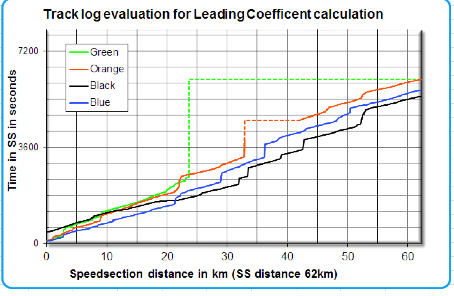
\includegraphics[scale=0.8]{img/leading-area.png}
    \caption{Sample track log graphs for \(LC\) calculation}
\end{figure}

\subsubsection{Example}
Blue was the first to enter the speed section, but Black was the first pilot to
cross the end of speed section. Green started at the same time as Blue, but
landed short, after about 23km and just over 40 minutes of flight inside the
speed section.

Black was fastest, therefore will get the most time points, but he started
late, probably had pilots out front to show the way during the first 22km, but
was leading after that.

If a pilot lands along the course (Green), or if his track log is interrupted
(Orange), his track log is completed as shown by the dotted lines: Missing
parts are calculated as if the dotted line was the actual track log, so LC
becomes bigger, lowering the leading points for that pilot, compared to a track
where that part is not missing. A pilot landing just short of goal will be less
penalised and could even get full leading points if he led for a long while.

The pilot who used best the earliest part of the day (i.e. Black, who has the
smallest area below the track log graph) gets all the available leading points,
while the others gets their points according to the same formula used for the
time points for the same reasons. If the task in the example is fully valid,
and 30\% of pilots reached goal, then Black will get all of the available 81
leading points and full time points, as he was fastest; Blue gets 45 leading
points because he started early but was slower; Orange receives only 18 leading
points as he was slow and had a gap in his track log; Green gets 0 points even
though he started early, because he was the slowest and landed fairly short.

\subsection{Arrival points}
\label{sec:arrival-points}
\begin{hg}
Arrival points depend on the position at which a pilot crosses ESS: The first
pilot completing the speed section receives the maximum available arrival
points, while the others are awarded arrival points according to the number of
pilots who reached ESS before them. The last pilot to reach ESS will always
receive at least 20\% of the available arrival points.
\begin{align*}
    AC_p &= 1 - \frac{PositionAtESS - 1}{NumberOfPilotsReachingESS} \\
    ArrivalFraction_p &= 0.2 + 0.037 * AC_p + 0.13 * AC_p^2 + 0.633 * AC_p^3 \\
    ArrivalPoints_p &= ArrivalFraction_p * AvailableArrivalPoints
\end{align*}
\end{hg}

\begin{figure}[h]
    \centering
    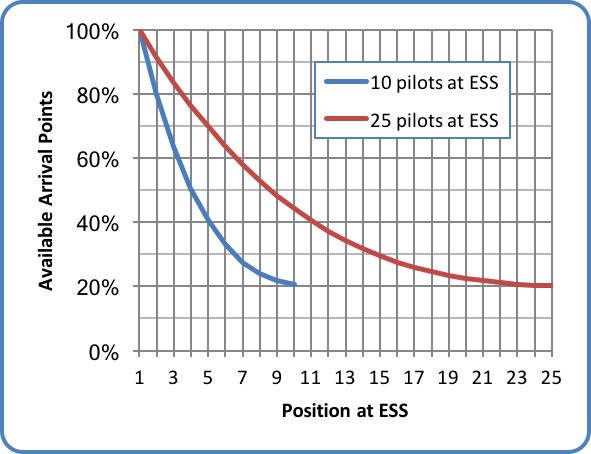
\includegraphics[scale=0.8]{img/arrival-points.png}
    \caption{Sample arrival points distributions}
\end{figure}

\begin{pg}
No arrival points are awarded in Paragliding.
\end{pg}

\newpage
\section{Special cases}
\label{sec:special-cases}
\subsection{ESS but not goal}
In a task where ESS and goal are not identical, a pilot may reach ESS, but not
goal. The way this case is handled differs between hang-gliding and paragliding
competitions:

\begin{pg}
In paragliding competitions, reaching goal is seen as “validating” one’s speed
section performance. A pilot who does not reach goal after reaching ESS will
lose his time points. He will only score distance points for the distance
actually covered, and leading points. This is seen as a safety measure, since
it encourages pilots to plan their final glide to ESS with enough altitude to
safely reach goal. This discourages high-speed final glides low to the ground.
\begin{align*}
    \forall p : p \in PilotsLandedBetweenESSandGoal : TotalScore_p &= \\
    DistancePoints_p + LeadingPoints_p + 0 * (TimePoints_p + ArrivalPoints_p)
\end{align*}
\end{pg}

\begin{hg}
In hang-gliding competitions, landing between ESS and goal is seen as a slight
mishap, which incurs a penalty on the pilot’s total score: Of the time and
arrival points scored on the speed section, the pilot will only receive
80\%\footnotemark
\begin{align*}
    \forall p : p \in PilotsLandedBetweenESSandGoal : TotalScore_p &= \\
    DistancePoints_p + LeadingPoints_p + 0.8 * (TimePoints_p + ArrivalPoints_p)
\end{align*}
\end{hg}
\footnotetext{Note that this „rule” is not defined in S7A, but is implemented
in FS. Some clarification on the rightfulness of this will be required.}.

\subsection{Early start}
\label{sec:early-start}
An early start occurs if a pilot’s last SSS cylinder boundary crossing in start
direction (enter or exit) occurred before the first (or only) start gate time.

\begin{pg}
In paragliding, pilots who perform an early start are only scored for the
distance between the launch point and the SSS cylinder, as calculated when
determining the complete task distance (see ~\ref{sec:task-distance}).
\end{pg}

\begin{hg}
In hang-gliding, the so-called “Jump the Gun”-rule applies: If the early start
occurred within a time that is close to the first (or only) start gate time,
the pilot is scored for his complete flight, but a penalty is then applied to
his total score.

The penalty calculation is based on two values X and Y, which are set in S7A,
but can be changed at the task briefing (presumably by the meet director and/or
the task committee). For each X seconds a pilot starts early, he incurs
a 1 point penalty, up to a maximum of Y seconds. If a pilot starts more than
Y seconds early, he will only be scored for minimum distance.
\begin{align*}
    X_{default} &= 2 \\
    Y_{default} &= 300 \\
    timeDiff_p &= firstStartGateTime - lastStartTime_p \\
    timeDiff_p \leq 0 : jumpTheGunPenalty_p &= 0 \\
    timeDiff_p > Y : jumpTheGunPenalty_p &= 0, totalScore_p = scoreForMinDistance \\
    0 < timeDiff_p \leq Y : jumpTheGunPenalty_p &= \frac{timeDiff_p}{X} \\
    \\
    totalScore_p &= \\
    \max(totalScore_p - jumpTheGunPenalty_p, scoreForMinDistance)
\end{align*}
\end{hg}

\subsection{Stopped tasks}
\label{sec:stopped-tasks}
\subsubsection{Stop task time}
\label{sec:stop-task-time}
A task can be stopped at any time by the meet director. The time when a stop
was announced for the first time is the “task stop announcement time”. This
time must be recorded to score the task appropriately. For scoring purposes,
a “task stop” time is calculated. This is the time which determines whether
a task will be scored at all. Pilots’ flight will only be scored up to this
task stop time.

\begin{hg}
In hang-gliding, stopped tasks are “scored back” by a time that is determined
by the number of start gates and the start gate interval: The task stop time is
one start gate interval, or 15 minutes in case of a single start gate, before
the task stop announcement time.
\begin{align*}
    numberOfStartGates = 1 : taskStopTime &= taskStopAnnouncementTime - 15min \\
    numberOfStartGates > 1 : taskStopTime &= taskStopAnnouncementTime - startGateInterval \\
\end{align*}
\end{hg}

\begin{pg}
In paragliding the score-back time is set as part of the competition parameters
(see section ~\ref{sec:score-back-time}).
\begin{align*}
    taskStopTime &= taskStopAnnouncementTime - competitionScoreBackTime \\
\end{align*}
\end{pg}

\subsubsection{Requirements to score a stopped task}
For a stopped task to be scored, it must fulfil certain requirements, which
differ between the two disciplines:

\begin{hg}
In hang gliding, a stopped task can only be scored if either a pilot reached
goal or the race had been going on for a certain minimum time. The minimum time
depends on whether the competition is the Women’s World Championship or not.
The race start time is defined as the time when the first valid start was taken
by a competition pilot.
\begin{align*}
    typeOfCompetition = Women's : minimumTime &= 60min \\
    typeOfCompetition \neq Women's : minimumTime &= 90min \\
    \\
    taskStopTime - timeOfFirstStart < minimumTime \land numberOfPilotsInGoal(taskStopTime) = 0 : \\
    taskValidity &= 0
\end{align*}
Note that this rule is currently not enforced by FS: The decision whether
a stopped task is cancelled or scored must be taken by the score keeper.
\end{hg}

\begin{pg}
In paragliding, a stopped task will be scored if the flying time was one hour
or more. For Race to Goal tasks, this means that the Task Stop Time must be one
hour or more after the race start time. For all other tasks, in order for them
to be scored, the task stop time must be one hour or more after the last pilot
started.
\begin{align*}
    minimumTime &= 60min \\
    \\
    typeOfTask = RaceToGoal \land numberOfStartGates = 1 : \\
    taskStopTime - startTime < minimumTime : \\
    taskValidity &= 0 \\
    \\
    typeOfTask \neq RaceToGoal \lor numberOfStartGates > 1 : \\
    taskStopTime - \max(\forall p : p \in StartedPilots . startTime_p) < minimumTime : \\
    taskValidity &= 0
\end{align*}
\end{pg}

\subsubsection{Stopped task validity}
For stopped tasks, an additional validity value, the Stopped Task Validity, is
calculated and applied to the Task Validity.
\[ DayQuality_{stopped} = LaunchValidity * DistanceValidity * TimeValidity * StoppedTaskValidity \]
Stopped Task Validity is calculated taking into account the task distance, the
flown distances of all pilots, the number of launched pilots and the number of
pilots still flying at the time when the task was stopped.
\begin{align*}
    NumberOfPilotsReachedESS > 0 : StoppedTaskValidity &= 1 \\
    NumberOfPilotsReachedESS = 0 : StoppedTaskValidity &= \min(1, a + b^3) \\
\end{align*}
\begin{align*}
    a &= \sqrt{\frac{BestDistFlown - avg(\forall i : DistFlown_i)}{DistLaunchToESS - BestDistFlown + 1} * \sqrt{\frac{stddev(\forall i : DistFlown)}{5}}} \\
    b &= \frac{NumPilotsLandedBeforeStopTime}{NumPilotsLaunched}
\end{align*}

\subsubsection{Scored time window}
For stopped Race to Goal tasks with a single start gate, scoring considers the
same time window for all pilots: The time between the race start and the task
stop time.
\begin{align*}
    typeOfTask = RaceToGoal \land numberOfStartGates = 1 : \forall p : p \in StartedPilots : \\
    scoreTimeWindow_p &= (startTime, taskStopTime)
\end{align*}
For stopped Race to Goal tasks with multiple start gates, as well as Elapsed
Time races, must be treated slightly differently: Only the time window
available to the last pilot started is considered for scoring. This time window
is defined as the amount of time t between the last pilot’s start and the task
stop time. For all pilots, only this time t after their respective start is
considered for scoring.
\begin{align*}
    typeOfTask \neq RaceToGoal \lor numberOfStartGates > 1 : \\
    scoreTime = taskStopTime - \max(\forall p : p \in StartedPilots : startTime_p) : \\
    \forall p : p \in StartedPilots : \\ 
    scoreTimeWindow_p &= (startTime_p, startTime_p + scoreTime)
\end{align*}
This means that if the last pilot started and then flew for, for example, 75
minutes until the task was stopped, all tracks are only scored for the first 75
minutes each pilot flew after taking their respective start.

\subsubsection{Time points for pilots at or after ESS}
Pilots who were at a position between ESS and goal at the task stop time will
be scored for their complete flight, including the portion flown after the task
stop time. This is to remove any discontinuity between pilots just before goal
and pilots who had just reached goal at task stop time.

\begin{pg}
If a Conical ESS is used, then all pilots who have crossed into the cone before
or at the task stop time will be scored for being in goal.
\end{pg}

A fixed amount of points is subtracted from the time points of each pilot that
makes goal in a stopped task. This amount is the amount of time points a pilot
would receive if he had reached ESS exactly at the task stop time. This is to
remove any discontinuity between pilots just before ESS and pilots who had just
reached ESS at task stop time.
\begin{align*}
    typeOfTask = RaceToGoal \land numberOfStartGates = 1 : \\
    timePointsReduction &= timePoints(taskStopTime - startTime) \\
    \\
    typeOfTask \neq RaceToGoal \lor numberOfStartGates > 1 : \\
    timePointsReduction &= \\
    timePoints(taskStopTime - \max(\forall p : p \in StartedPilots : startTime_p)) \\
    \\
    \forall p : p \in PilotsInGoal : finalTimePoints_p &= timePoints_p - timePointsReduction
\end{align*}

\subsubsection{Distance points with altitude bonus}
\label{sec:distance-stopped-tasks}
To compensate for altitude differences at the time when a task is stopped,
a bonus distance is calculated for each point in the pilots’ track logs, based
on that point’s altitude above goal. This bonus distance is added to the
distance achieved at that point. All altitude values used for this calculation
are GPS altitude values, as received from the pilots’ GPS devices (no
compensation for different earth models applied by those devices). For all
distance point calculations, including the difficulty calculations in
hang-gliding (see ~\ref{sec:difficulty-calculation}), these new stopped
distance values are being used to determine the pilots’ best distance values.
Time and leading point calculations remain the same: they are not affected by
the altitude bonus or stopped distance values.
\begin{align*}
    \hgh{GlideRatio} &= 5.0 \\
    \pgh{GlideRatio} &= 4.0 \\
    \forall p : p \in PilotsLandedBeforeGoal : bestDistance_p &= max(minimumDistance, taskDistance - \min(xs)) \\
    \forall p : p \in PilotsReachedGoal : bestDistance_p &= taskDistance
\end{align*}
\[ xs = \forall track_p . point_i : shortestDistanceToGoal(track_p . point_i) - (track_p . point_i . altitude - GoalAltitude) * GlideRatio \\ \]

\subsection{Penalties}
Penalties for various actions are defined in the rules. These penalties are
either expressed as an absolute number (e.g. “100 points”) or as a percentage
(e.g. “10\% of the pilot’s score in the task where he performed the punishable
action”). The corresponding number of points is then deducted from the punished
pilot’s total score to calculate his final score.
\begin{align*}
    finalScore_p &= score_p - absolutePenalty \\
    finalScore_p &= score_p - (1 - percentagePenalty_p)
\end{align*}

\begin{hg}
These penalties are completely independent of any “Jump the Gun”-Penalty
a pilot may have incurred.
\end{hg}

The penalty mechanism can also be used to award bonus points to a pilot for
some actions like helping a pilot in distress. In that case the penalty must be
given as a negative number.

Any rounding up of scores is to be done after the application of penalties. The
lowest score a pilot can attain in a task, regardless of any incurred
penalties, is zero points.

\newpage
\section{Task ranking}
\label{sec:task-ranking}
\subsection{Overall task ranking}
Pilots are ranked by their final score, in descending order. Pilots with the
same score are ranked in the same position.

\subsection{Female task ranking}
A female task ranking is generated by exclusively listing female pilots, with
the score they achieved in the overall task ranking. Female pilots with the
same score are ranked in the same position.

\subsection{Nation task ranking}
\begin{hg}
For the nation task ranking, except for the Women’s World Championships, the
scores of the three best-ranked pilots of each national team are added up to
create each nation’s task score. For the nation task ranking at the Women’s
World Championships, the scores of the two best-ranked pilots of each national
team are added up to create each nation’s task score. The nations are then
ranked by their score, in descending order. Nations with the same score are
ranked in the same position.
\end{hg}

\begin{pg}
For the nation task ranking, the scores of the two best-ranked pilots of each
national team are added up to create each nation’s task score. The nations are
then ranked by their score, in descending order. Nations with the same score
are ranked in the same position.
\end{pg}

\newpage
\section{Competition ranking}
\label{sec:competition-ranking}
\subsection{Overall competition ranking}
\label{sec:overall-competition-ranking}
\begin{hg}
The competition overall score of a pilot is calculated by adding up all of his
task scores. Pilots are then ranked according to their overall total score, in
descending order, for the overall competition ranking. Pilots with the same
score are ranked in the same position.
\end{hg}

\begin{pg}
The overall score of a pilot is calculated by using the FTV algorithm described
in section~\ref{sec:fixed-total-validity}. For competitions with up to
6 planned tasks, an FTV factor of 0.2 is used. For competitions with 7 or more
planned tasks, an FTV factor of 0.25 is used. Pilots are then ranked according
to their overall score, in descending order, for the overall competition
ranking.\footnotemark
\end{pg}
\footnotetext{Organisers of Category 2 competitions are free to choose
whether they want to use FTV for overall scores. Especially for shorter
competitions with fewer than 4 tasks, using the traditional method (adding up
all task scores for each pilot) may be more suitable.}

\subsection{Female competition ranking}
The female competition ranking is generated by exclusively listing female
pilots, with the score they achieved in the overall competition ranking.

\subsection{Nation competition ranking}
The competition score of a nation is calculated by adding up all of that
nation’s task scores. Nations are then ranked according to their competition
total score, in descending order, for the nation competition ranking.

\subsection{Ties}
If the scores of the first, second or third in the overall, female or nation
ranking are identical, the tie shall be broken by adding up the task positions
of the tied pilots, or teams. The pilot or team with the lowest sum is declared
the winner. If this does not break the tie, joint champions will be declared.
For all other ranking positions, pilots or nations with the same score are
ranked in the same position.

\newpage
\section{FTV - Fixed Total Validity}
\label{sec:fixed-total-validity}
Fixed Total Validity (FTV) is a procedure to score pilots on their best task
performances, rather than all their tasks. Fixed Total Validity means the sum
(total) of available points (validity) is set (fixed) to the same value for
each competitor.
\begin{align*}
    FTVfactor &= 0.2 \lor 0.25 \\
    CalculatedFTV &= (1 - FTVfactor) * \sum_{t : Task}\frac{AvailablePoints_t}{1000}
\end{align*}
To calculate a pilot’s FTV score, for all his flights:
\begin{enumerate}
    \item
        Calculate a performance percentage for each day by dividing the pilot's
        day score by the day’s available points
    \item
        Arrange all flights in descending order of performance percentage
    \item
        Total up the flights' raw day scores (not performance percentages) in
        order of performance percentage until the sum of validities for those
        scores reaches the pre-decided Fixed Total Validity value.
\end{enumerate}
If the last score added takes that pilot's total validity above the Fixed Total Validity, then only a fraction
of that score is used so that the pilot's total validity is equal to the Fixed Total Validity.
\begin{align*}
    \forall t : t \in ScoredTasks : Performance_{p, t} &= \frac{Score_{p, t}}{AvailablePoints_t} \\
    \\
    SortedPerformance_p &= sortDescending(\forall t : t \in ScoredTasks : Performance_{p, t}) \\
    \\
    OrderedValidities_p &= orderByPerformance(SortedPerformance_p, xs) \\
    xs &= \forall t : t \in ScoredTasks : \frac{AvailablePoints_t}{1000} \\
    \\
    OrderedScores_p &= orderByPerformance(SortedPerformance_p, ys) \\
    ys &= \forall t : t \in ScoredTasks : Score_{p, t} \\
    \\
    FTVScore_p &= \sum_{u = 0}^{numberOfTasks} OrderedScores_{p, u} * \max(1, \frac{\min(0, a)}{OrderValidites_{p, u}}) \\
    a &= CalculatedFTV - (u > 0 : \sum_{v = 0}^{\min(0, u - 1)} OrderedValidites_{p, v})
\end{align*}

\end{document}
